\section{二次曲面用谱分解显露几何形状}
\label{sec:03-Linear-Algebra/06-Symmetric-and-Positive-Definite-Matrices/04}

有人递给你两个可行域，问哪个是有界的：

\[
5x^2+4xy+2y^2\le1,
\qquad
5x^2+4xy+0.5y^2\le1 .
\]

两个式子只差一个系数。第一个是一片倾斜的椭圆盘，面积有限；第二个是一对张开到无穷远的双曲区域，在里面往某些方向走多远都不会越界。肉眼分不出来，画图前也猜不准，因为交叉项 \(4xy\) 把形状藏起来了。

判据在上一节其实已经准备好。写成矩阵形式，两者对应

\[
A_1=\begin{pmatrix}5&2\\2&2\end{pmatrix},
\qquad
A_2=\begin{pmatrix}5&2\\2&0.5\end{pmatrix},
\]

\(\det A_1=6>0\) 且迹为正，两个特征值同号且为正；\(\det A_2=-1.5<0\)，一正一负。前者是碗，后者是鞍。本节把这条判据推到一般的二次方程

\[
x^{\trans}Ax+2b^{\trans}x+c=0,\qquad A=A^{\trans},
\]

并说明为什么``看起来像''从来不是可靠的分类方式。

\subsection{旋转拿走交叉项}

交叉项之所以出现，多半只是因为坐标轴没有摆在图形的主方向上。谱定理正好提供了摆正的方式：取 \(A=Q\Lambda Q^{\trans}\)，令 \(z=Q^{\trans}x\)，则

\[
x^{\trans}Ax=z^{\trans}\Lambda z=\sum_{i=1}^{n}\lambda_iz_i^2 .
\]

\(Q\) 正交，这次换坐标只是旋转或反射，长度与夹角一分未动，所以``图形本身''没有被改变，改变的只是我们看它的角度。

\begin{center}
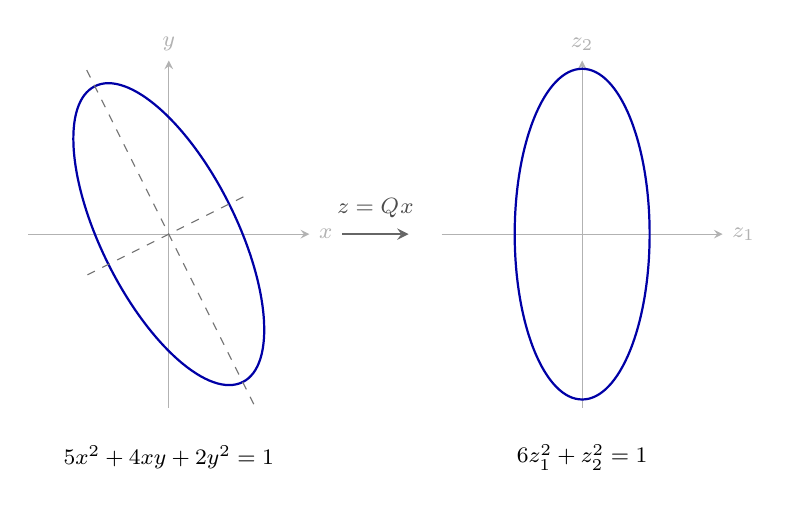
\begin{tikzpicture}[x=2.1cm,y=2.1cm,font=\small,>=stealth]
  \draw[black!30,->] (-0.85,0) -- (0.85,0) node[right,font=\footnotesize] {\(x\)};
  \draw[black!30,->] (0,-1.05) -- (0,1.05) node[above,font=\footnotesize] {\(y\)};
  \begin{scope}[rotate=26.565]
    \draw[blue!65!black,thick] (0,0) ellipse (0.408 and 1);
    \draw[black!55,dashed] (-0.55,0) -- (0.55,0);
    \draw[black!55,dashed] (0,-1.15) -- (0,1.15);
  \end{scope}
  \node[font=\footnotesize] at (0,-1.35) {\(5x^2+4xy+2y^2=1\)};
  \draw[->,thick,black!60] (1.05,0) -- (1.45,0);
  \node[above,black!70,font=\footnotesize] at (1.25,0.04) {\(z=Q^{\trans}x\)};
  \begin{scope}[shift={(2.5,0)}]
    \draw[black!30,->] (-0.85,0) -- (0.85,0) node[right,font=\footnotesize] {\(z_1\)};
    \draw[black!30,->] (0,-1.05) -- (0,1.05) node[above,font=\footnotesize] {\(z_2\)};
    \draw[blue!65!black,thick] (0,0) ellipse (0.408 and 1);
    \node[font=\footnotesize] at (0,-1.35) {\(6z_1^2+z_2^2=1\)};
  \end{scope}
\end{tikzpicture}

\emph{同一条椭圆的两幅画像。左边虚线是 \(A\) 的两条特征方向，分别沿 \((2,1)^{\trans}\) 与 \((1,-2)^{\trans}\)；右边把坐标轴转到这两条线上，交叉项消失。半轴长是 \(1/\sqrt{\lambda_i}\)：特征值 6 的方向短，特征值 1 的方向长。}
\end{center}

半轴与特征值的这层倒数关系值得单独记一次。本单元第一节里那张圆变椭圆的图上，\(A\) 把单位圆拉长的方向是特征值大的方向；这里等高线被压短的方向同样是特征值大的方向。两句话不矛盾——特征值大意味着同样的位移换来更多的能量，所以要维持 \(x^{\trans}Ax=c\) 不变，就只能走得更近。看图时先确认画的是像还是等高线。

\subsection{平移找到中心，分类只剩符号}

线性项 \(2b^{\trans}x\) 只是把图形挪离原点。\(A\) 可逆时取 \(x_0=-A^{-1}b\) 并令 \(x=x_0+u\)，配方后线性项消失：

\[
x^{\trans}Ax+2b^{\trans}x+c=u^{\trans}Au+c-b^{\trans}A^{-1}b .
\]

再旋转一次，令 \(z=Q^{\trans}u\)，整个方程化为

\[
\sum_i\lambda_iz_i^2=d,\qquad d=b^{\trans}A^{-1}b-c .
\]

到这一步分类不再需要想象力。特征值全部同号且 \(d\) 与之匹配时是椭球型，有界闭合；出现一正一负时是双曲型，无界；\(d\) 符号与全同号的特征值相反时集合是空的。

零特征值要单独处理，因为那些方向上 \(A\) 不可逆，上面的配方做不了。留下来的线性项若在零方向上非零，图形沿该方向被抛物线状地推出去，得到抛物型；若线性项在零方向上也为零，方程退化成平面、直线、锥面或空集。这正是``看起来像''最容易翻车的地方：\(x^2+y^2=0\) 在实平面上只有一个点，可它的写法和一族圆完全同形。

于是回到开头。\(5x^2+4xy+2y^2\le1\) 的矩阵有两个正特征值，是椭圆盘，只是主轴相对坐标轴转了 \(\arctan(1/2)\)；把 2 换成 0.5 之后行列式变负，同样的写法给出双曲区域。判断有界性只需要两个特征值的符号，甚至只需要行列式与迹。眼睛在这件事上帮不上忙，代数可以。

\subsection{误差椭圆把这套几何搬进测量}

定位、标定、参数估计给出的结果通常是一个中心 \(\widehat x\) 加一个协方差矩阵 \(\Sigma\)。把等马氏距离的点集画出来，

\[
(x-\widehat x)^{\trans}\Sigma^{-1}(x-\widehat x)=r^2,
\]

就是误差椭圆。\(\Sigma\) 半正定，\(\Sigma^{-1}\) 在可逆时也正定，所以这条曲线必是椭圆——上一段的分类在这里退化成一句必然。

\begin{center}
\begin{tikzpicture}[x=1.1cm,y=1.1cm,font=\small,>=stealth]
  \draw[black!25,->] (-2.4,0) -- (2.4,0) node[right,font=\footnotesize] {\(x_1\)};
  \draw[black!25,->] (0,-2.4) -- (0,2.4) node[above,font=\footnotesize] {\(x_2\)};
  \draw[black!45,dashed] (-1,-1) rectangle (1,1);
  \begin{scope}[rotate=45]
    \draw[blue!65!black,thick] (0,0) ellipse (1.342 and 0.447);
    \draw[blue!45!black] (0,0) ellipse (2.683 and 0.894);
    \draw[->,black!70] (0,0) -- (1.342,0);
    \draw[->,black!70] (0,0) -- (0,0.447);
  \end{scope}
  \fill (0,0) circle (2pt);
  \node[font=\footnotesize] at (2.9,1.95) {\(\sqrt{\lambda_1}=1.34\)};
  \node[font=\footnotesize] at (-2.0,1.45) {\(\sqrt{\lambda_2}=0.45\)};
  \node[below,font=\footnotesize] at (0,-2.9) {\(\Sigma=\bigl(\begin{smallmatrix}1&0.8\\0.8&1\end{smallmatrix}\bigr)\)};
\end{tikzpicture}

\emph{上一节那批点云的两条误差椭圆（\(r=1\) 与 \(r=2\)）。两条主轴由 \(\Sigma\) 的特征向量给出，半轴长是 \(r\sqrt{\lambda_i}\)。虚线方框的边长由两个边缘标准差决定，都等于 1；\(1\sigma\) 椭圆恰好内切于它。方框对相关性一无所知，倾斜的那部分信息全在椭圆里。}
\end{center}

图里那个方框值得多说一句。报告参数不确定性时若只给每个分量的标准差，读者拿到的就是那个方框；而真实的联合不确定性是里面那条细长的椭圆。两者在坐标轴方向上一样宽，在 \((1,1)^{\trans}\) 与 \((1,-1)^{\trans}\) 方向上差了三倍。忽略非对角元，等于把一条清楚的窄脊报告成一片模糊的方块。

\(\Sigma\) 的谱分解在这里同时给出三样东西：特征向量是椭圆的倾斜方向，特征值的平方根是各主轴上的典型误差尺度，条件数是椭圆的扁平程度——也就是哪一个方向的参数被数据管住了、哪一个几乎没被约束。这跟 PCA 是同一套计算，只不过那边把大特征值方向当作信号，这边把大特征值方向当作最不确定的那个方向。

边界也清楚。\(\Sigma\) 奇异时 \(\Sigma^{-1}\) 不存在，椭球在零特征值方向上``无限薄''，说明数据实际落在一个低维子空间里。正确的做法是在有效子空间内用伪逆，把退化方向如实报告成``该方向没有信息''，而不是为了套公式给每个方向硬凑一点不确定性。

\subsection{同一套几何还会在哪里出现}

本单元的三件事在这里合流：谱定理挑出正交的主轴，二次型读出每条主轴上的尺度，正定性判断这张能量面是碗还是鞍。

多元高斯的密度是 \(\exp(-\frac12u^{\trans}\Sigma^{-1}u)\)，等密度面就是误差椭球，采样时用 Cholesky 的 \(L\) 把球形噪声塑成它。二次优化的等高线是同一族椭球，条件数决定一阶方法要绕多少圈。Newton 法在每一步用局部 Hessian 造一个椭球模型并跳到它的中心，信赖域方法则给这个模型加一个球形或椭球形的活动范围。回归的置信区域、卡尔曼滤波的不确定性传播、GP 后验的方差带，画出来都是这条椭圆在不同坐标下的样子。

判断一个新场景是否属于这一类，只要问两件事：目标里的二阶项是不是写成了 \(x^{\trans}Ax\)，那个 \(A\) 是不是正定。第一件决定几何是椭球族，第二件决定它闭不闭合。答案都为是的时候，本单元的全套工具可以原样搬过去；有一个为否，就先回到上一节看能量在哪个方向上漏掉了。
